\documentclass[11pt,a4paper]{scrartcl}
\usepackage[top=3cm,bottom=3cm,left=2cm,right=2cm]{geometry} % Seitenränder einstellen
\usepackage[utf8]{inputenc} % Umlaute im Text
\usepackage[english]{babel} % Worttrennung nach der neuen Rechtschreibung und deutsche Bezeichnungen
\usepackage[dvipsnames]{xcolor} % Farbe in Dokument
\parindent 0pt % kein Einrücken bei neuem Absatz
\usepackage{amsmath} % zusätzliche mathematische Umgebungen
\usepackage{amssymb} % zusätzliche mathematische Symbole
%\usepackage{bbold} % zusätzliche mathematische Symbole
\usepackage{units} % schöne Einheiten und Brüche
\usepackage{icomma} % kein Leerzeichen bei 1,23 in Mathe-Umgebung
\usepackage{wrapfig} % von Schrift umflossene Bilder und Tabellen
\usepackage{picinpar} % Objekt in Fließtext platzieren (ähnlich zu wrapfig)
\usepackage{scrhack} % verbessert andere Pakete, bessere Interaktion mit KOMA-Skript
\usepackage{float} % bessere Anpassung von Fließobjekten
\usepackage{pgf} % Makro zur Erstellung von Graphiken
\usepackage{tikz} % Benutzeroberfläche für pgf
\usepackage[margin=10pt,font=small,labelfont=bf,labelsep=endash,format=plain]{caption} % Einstellungen für Tabellen und Bildunterschriften
\usepackage{listings}
\usepackage{subcaption} % Unterschriften für mehrere Bilder
\usepackage{enumitem} % no indentation at description environment
\usepackage[onehalfspacing]{setspace} % Änderung des Zeilenabstandes (hier: 1,5-fach)
\usepackage{booktabs} % Einstellungen für schönere Tabellen
\usepackage{graphicx} % Einfügen von Grafiken -> wird in master-file geladen
\usepackage{url} % URL's (z.B. in Literatur) schöner formatieren
\usepackage[pdftex]{hyperref} % Verweise innerhalb und nach außerhalb des PDF; hyperref immer als letztes Paket einbinden

% define bordermatrix with brackets

\makeatletter
\def\bbordermatrix#1{\begingroup \m@th
  \@tempdima 4.75\p@
  \setbox\z@\vbox{%
    \def\cr{\crcr\noalign{\kern2\p@\global\let\cr\endline}}%
    \ialign{$##$\hfil\kern2\p@\kern\@tempdima&\thinspace\hfil$##$\hfil
      &&\quad\hfil$##$\hfil\crcr
      \omit\strut\hfil\crcr\noalign{\kern-\baselineskip}%
      #1\crcr\omit\strut\cr}}%
  \setbox\tw@\vbox{\unvcopy\z@\global\setbox\@ne\lastbox}%
  \setbox\tw@\hbox{\unhbox\@ne\unskip\global\setbox\@ne\lastbox}%
  \setbox\tw@\hbox{$\kern\wd\@ne\kern-\@tempdima\left[\kern-\wd\@ne
    \global\setbox\@ne\vbox{\box\@ne\kern2\p@}%
    \vcenter{\kern-\ht\@ne\unvbox\z@\kern-\baselineskip}\,\right]$}%
  \null\;\vbox{\kern\ht\@ne\box\tw@}\endgroup}
\makeatother

% make Titel
\title{Mining massive Datasets WS 2017/18}
\subtitle{Problem Set 2}
\author{Rudolf Chrispens, Marvin, Daniela Schacherer}

\begin{document}

\maketitle

	\section*{Exercise 01}
	
	
	See hand written solution. 
	\section*{Exercise 02}
	In order to also maintain information about which points are in which cluster one could store each Point p as \\
(\textit{vector sum of points in cluster, number of points in cluster, list of data points in the cluster}). \\

Pseudocode for step 3 and 4 of subroutine \textit{merge} from lecture 3:
	\begin{itemize}
		\item Find best pair, merge those two points/clusters and compute new cluster center\\
		d, (p,q), (ip, iq) = bestPair\\
		\textbf{sum} = p[0] + q[0] \\
		\textbf{count} = p[1] + q[1] \\
		\textbf{points} = p[2].append(q[2]) \\
		newCenter = (\textbf{sum}, \textbf{count}, \textbf{points}) \\

		\item Filter p and q from the inCluster
		\item Re-number centroid index in inCluster
		\item Add new cluster to the outCluster
		
	\end{itemize}


\section*{Exercise 03}

\lstset{breaklines=true}
\begin{enumerate}
\item The values we got (also at the end of the output):\\
SSE: 14.380579250974264\\
BCV/WCV: 0.17328857891525754\\\\
The complete output:
\begin{lstlisting}
['/home/immd-user/IdeaProjects/immd-project-example/kmeans-IMMD-lecture2.py', '100', '3', '0.015'] # test parameter
Number of points: 100

### Iteration#: 0
Cluster with index 0 has 9 points
Cluster with index 1 has 14 points
Cluster with index 2 has 77 points
*tempDist=0.404830
*centroids=[array([-0.76598659, -0.52866356]), array([-0.76547008, -0.41186522]), array([-0.38506119, -0.50170466])]
*newCentroids=[array([-0.74211243, -0.65927882]), array([-0.71465718, -0.1472639 ]), array([ 0.17123155, -0.42999355])]

### Iteration#: 1
Cluster with index 0 has 23 points
Cluster with index 1 has 20 points
Cluster with index 2 has 57 points
*tempDist=0.088571
*centroids=[array([-0.74211243, -0.65927882]), array([-0.71465718, -0.1472639 ]), array([ 0.17123155, -0.42999355])]
*newCentroids=[array([-0.5857041 , -0.66901706]), array([-0.56997999, -0.11177287]), array([ 0.37493704, -0.41196241])]

### Iteration#: 2
Cluster with index 0 has 29 points
Cluster with index 1 has 25 points
Cluster with index 2 has 46 points
*tempDist=0.031933
*centroids=[array([-0.5857041 , -0.66901706]), array([-0.56997999, -0.11177287]), array([ 0.37493704, -0.41196241])]
*newCentroids=[array([-0.50150539, -0.66017534]), array([-0.47765785, -0.09113332]), array([ 0.49968956, -0.42785412])]

### Iteration#: 3
Cluster with index 0 has 30 points
Cluster with index 1 has 27 points
Cluster with index 2 has 43 points
*tempDist=0.004239
*centroids=[array([-0.50150539, -0.66017534]), array([-0.47765785, -0.09113332]), array([ 0.49968956, -0.42785412])]
*newCentroids=[array([-0.50146902, -0.65085887]), array([-0.4275621 , -0.09255383]), array([ 0.53695034, -0.44372065])]

=== Final centers: [array([-0.50146902, -0.65085887]), array([-0.4275621 , -0.09255383]), array([ 0.53695034, -0.44372065])]

test partition:
SSE: 14.380579250974264
BCV/WCV: 0.17328857891525754

Process finished with exit code 0
\end{lstlisting}
\item We also uploaded the python file for this problem. We build a function for the k-means algorithm and call that function 20 times. At the end the plots are created.
\item The appropriate \textit{k} value is short after the big drop of the \textit{SSE} value what is something like 5.\\

Picture \ref{sse} (page 4) shows the SSE value. Of course at the beginning its pretty big because we have just one cluster and the points can be far away of the one centroid. But with higher \textit{k} the value sinks because there are more centroids and the distance to the points are shorter.\\

Picture \ref{bcv_wcv} (page 4) shows the BCV/WCV value. At the beginning it is zero because we just have one cluster with no distance to another. Then the value increases because the SSE sinks.
\end{enumerate}

\begin{figure}[htbp] 
  \centering
	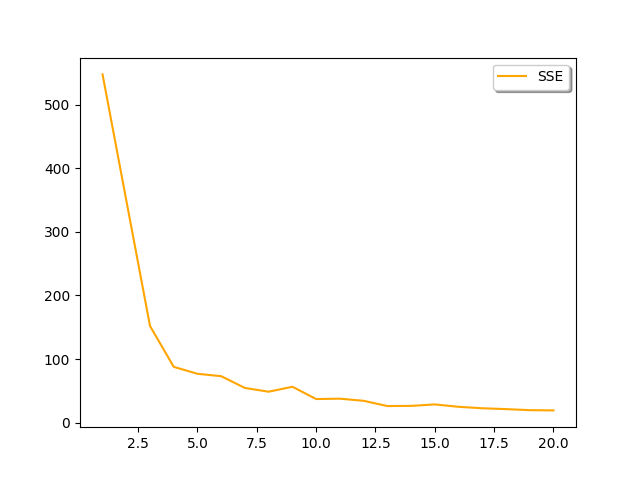
\includegraphics[width=0.75\textwidth]{sse.png}
  \caption{Exercise 3 - SSE}
  \label{sse}
\end{figure}

\begin{figure}[htbp] 
  \centering
	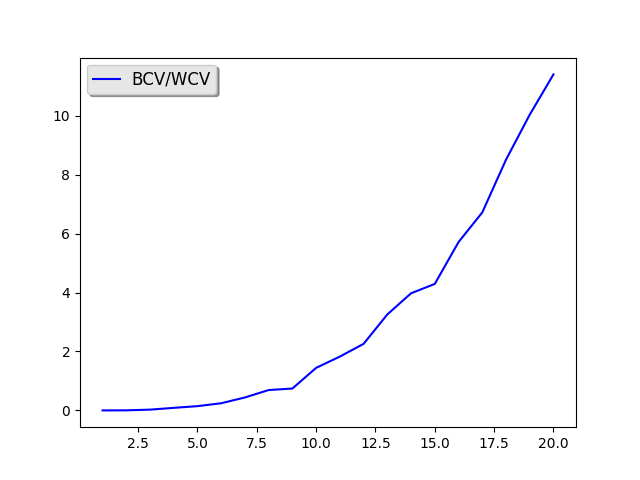
\includegraphics[width=0.75\textwidth]{bcv_wcv.png}
  \caption{Exercise 3 - BCV/WCV}
  \label{bcv_wcv}
\end{figure}


\section*{Exercise 04 - Pseudocode}
\paragraph{Step 1:}
Take a small sample of the data and cluster it in main memory.\\
In principle, any clustering method could be used, but as CURE is designed to handle oddly shaped clusters, it is often advisable to use a hierarchical method in which clusters are merged when they have a close pair of points.
\begin{tabbing}
Links \= Mitte \= Rechts \kill
\>	\#Take a Sample of the whole Dataset\\
\>	\#use hierarchical clustering algorithm to cluster the sampleData\\
\> \>	 sampleSize;\\
\> \> 	sampleData = textFile.takeSample(false, sampleSize);\\
\> \>	hierarchicalCluster = HclusterAlgorythm( sampleData );
\end{tabbing}
\paragraph{Step 2:}
Select a small set of points from each cluster to be representative points. \\
These points should be chosen to be as far from one another as possible, \\
using the method described in Section 7.3.2.
\begin{tabbing}
Links \= Mitte \= Rechts  \=Rechts2 \kill
\#Select small set of points of each cluster. \\
\#They should be as far as possible from each other\\
FOR EACH hCluster in hierarchicalCluster DO\\
\>\#Pick the first point at random\\
\>\>	repPoints.add( hCluster.takeSample(false, 1) );\\
\>WHILE repPoints.count() $<$ hierarchicalCluster.count() DO\\
\>\#Add the point whose minimum distance from the selected points is as largest; \\
\>furthestPoint;\\
\>FOR EACH point in hCluster DO\\
\> \>		If( furthestPoint.squared\_distance( repPoints ) $<$ 
			Point.squared\_distance( repPoints ) ) DO\\
\> \>	\>		furthestPoint = point;\\
\>repPoints.add( furthestPoint);\\
END;
\end{tabbing}
\paragraph{Step 3:}
Move each of the representative points a fixed fraction of the distance between its location and the centroid of its cluster. Perhaps 20\% is a good fraction to choose. Note that this step requires a Euclidean space, since otherwise, there might not be any notion of a line between two points.

\begin{tabbing}
Links \= Mitte \= Rechts \kill
\> FOR EACH repPoint in repPoints DO\\
\> \> 	Center = clusterCenters(repPoints);\\
\> \> 	repPoint.moveTo(Center,0.2);
\end{tabbing}

\paragraph{Step 4:}
The next phase of CURE is to merge two clusters if they have a pair of representative points, one from each cluster, that are sufficiently close. The user may pick the distance that defines ?close.? This merging step can repeat, until there are no more sufficiently close clusters.
\begin{tabbing}
Links \= Mitte \= Rechts  \=Rechts2 \kill
\> 	Threshold;\\
\> 	FOR EACH cluster in repPoints DO\\
\> \> 		IF (closestClusterFound = closest\_cluster(repPoints, cluster, Threshold):\\
\> \> 	\>		mergeCluster(closestClusterFound, cluster):
\end{tabbing}
\paragraph{Step 5:}
The last step of CURE is point assignment. Each point p is brought from secondary storage and compared with the representative points. We assign p to the cluster of the representative point that is closest to p.
\begin{tabbing}
Links \= Mitte \= Rechts  \=Rechts2 \kill
\> FOR EACH point in Dataset DO\\
\> \>	nearestCluster(point, repPoints).add(point);
\end{tabbing}

\end{document}

